\subsubsubsubsection{UEBuilder}
\begin{figure}[h]
\centering
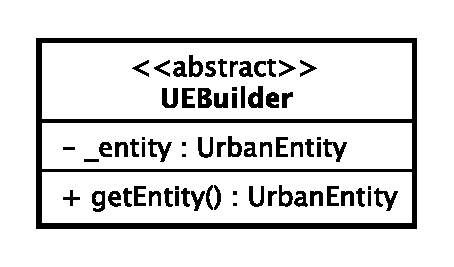
\includegraphics[scale=0.6,keepaspectratio]{images/solution/uebuilder.eps}
\caption{App::Reactive::UEBuilder}
\label{fig:sd-app-uebuilder}
\end{figure}
\FloatBarrier
\begin{itemize}
  \item \textbf{Description} \\
    It represents a component that builds urban entities like crossroads and
    streets.
  \item \textbf{Attribute}
  \begin{itemize}
    \item \texttt{- \_entity: UrbanEntity} \\
The entity which the builder incrementally constructs.
  \end{itemize}
  \item \textbf{Operation}
  \begin{itemize} 
    \item \texttt{+ getEntity() : UrbanEntity} \\
Returns the final product of the building.
  \end{itemize}
\end{itemize}
